\section{SunSPOT}\label{s:Sunspot}

Die Firma Oracle besitzt im Rahmen seiner Java-Technologie eine Vormachtstellung im Bereich der Smartphones.
Auf der Welt sind schätzungsweise über eine Milliarde Smartphones mit der Java-Technologie lizenziert. \cite{d:horan} \\ Ziel von Oracle ist es, auch in den zukunftsnahen Technologien mit ihrer Programmiersprache Java auszustatten und diese Produkte zu etablieren.\\

Ein erster Schritt in diese Richtung is das von Oracle entwickelte "'SunSPOT"'-Sensornetzwerk. SunSPOT bedeutet "'Sun Small Programmable Object Technology"' und ist eine Plattform für Java-basierte drahtlose Sensornetzwerke. Sie bestätigt den Trend, dass in immer kleiner werdenden Geräten zunehmend leistungsfähigere Technologien eingesetzt werden. Dabei ist wichtig, dass jene Geräte, am Besten drahtlos, miteinander kommunizieren können und jederzeit von überall auf der Welt steuerbar bleiben. Das SunSPOT Starter Paket besteht aus einer Basisstation und 2 Sensoren. \\

\begin{figure}[H] 
	\centering
	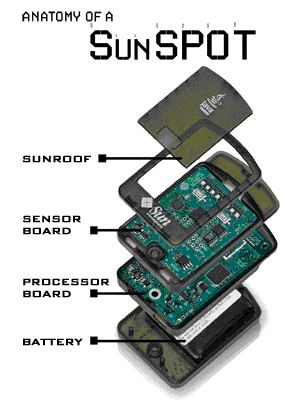
\includegraphics[scale=0.5]{Bilder/spotanatomy}
	\caption{Anatomie eines Standard SunSPOT-Sensors\cite{i:spotaufbau}}
	\label{f:spotaufbau}
\end{figure}

Die Hardware der SunSPOT-Sensoren ist modular aufgebaut. Das bedeutet, dass man die verfügbaren Boards frei nach Belieben aufeinander stecken und somit verbinden kann. Dabei können maximal bis zu 3 Boards + Stromversorgung miteinander verknüpft werden. \cite{d:horan} \\

\subsection{Technische Daten}\label{ss:TechnischeDaten}

Hier werden alle technischen Daten der SunSPOTS erklärt.